
\subsection{Class Diagram}
\vspace{1cm}
\begin{figure}[h]
    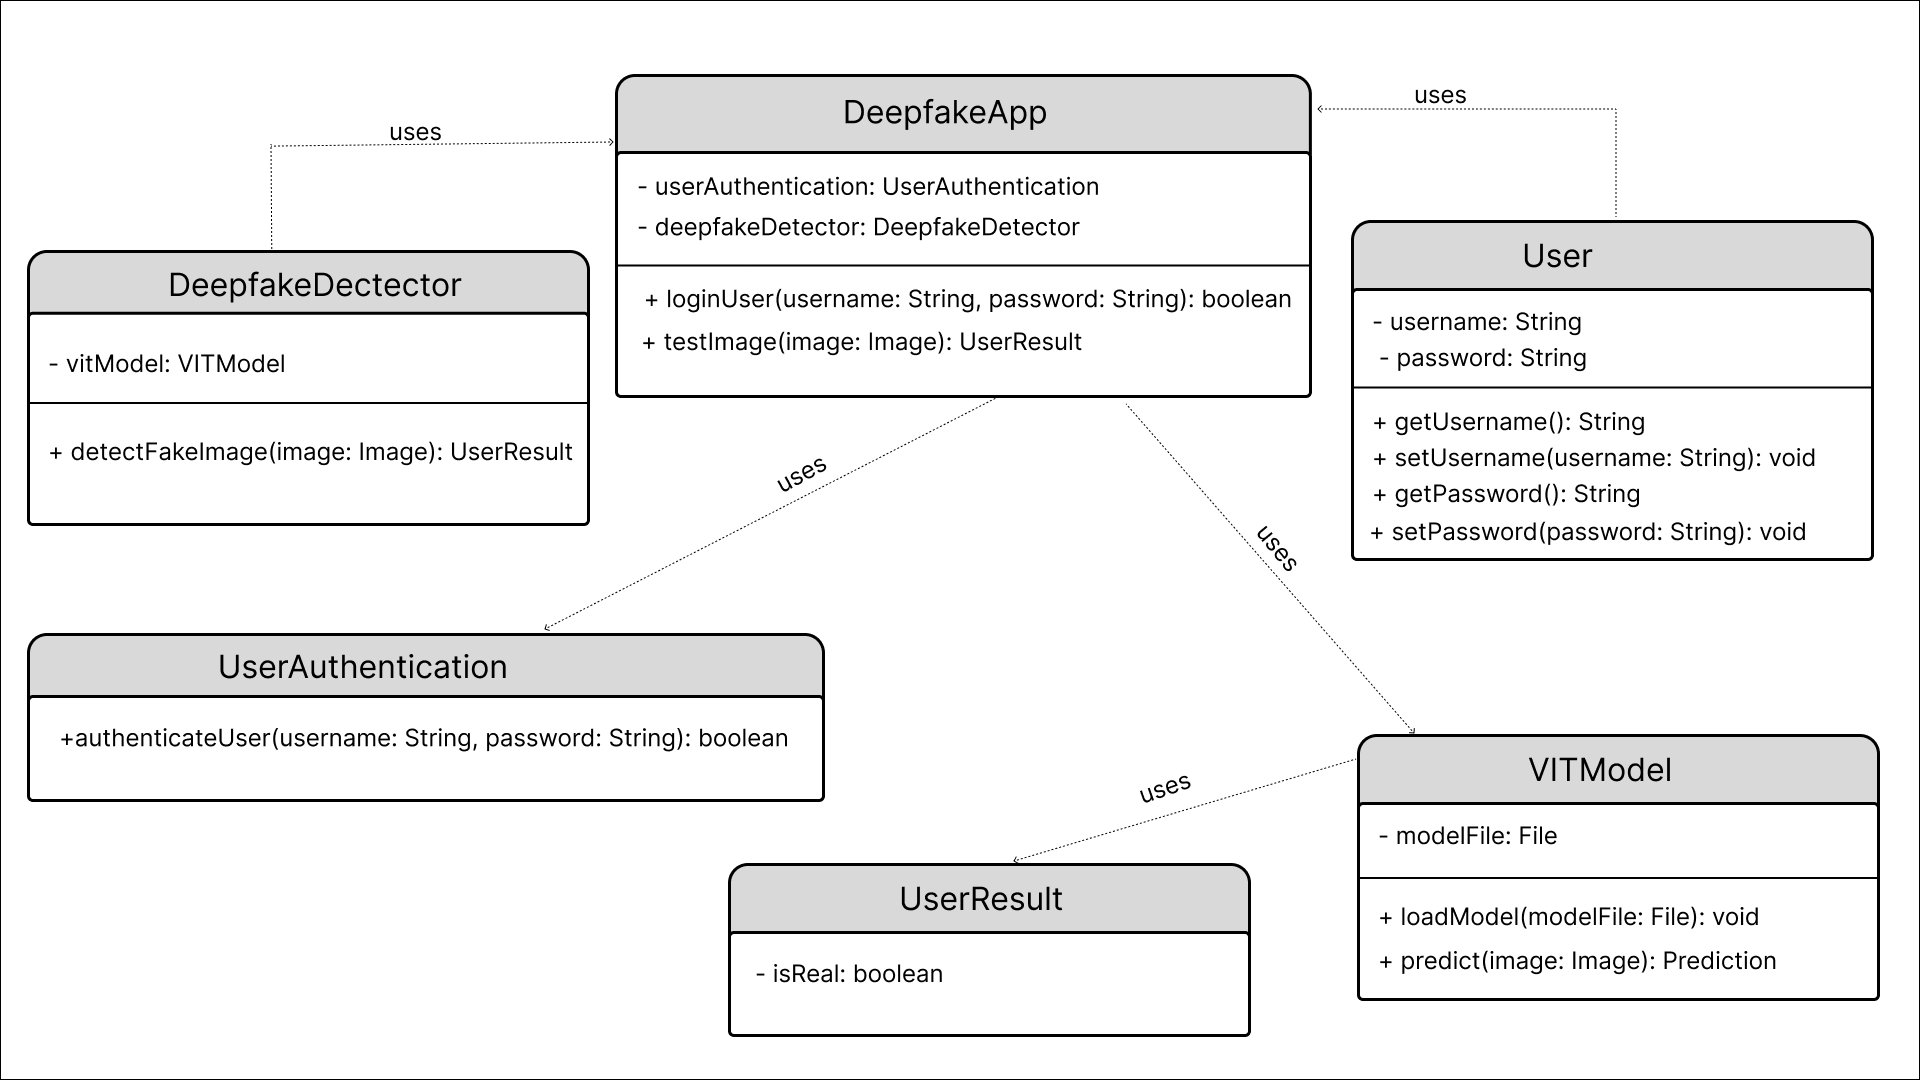
\includegraphics[width=1\textwidth,height=6in,keepaspectratio]{img/classdiagram.jpg}
    \caption{{Class Diagram}}
\end{figure}

\justify
The class diagram for our deepfake detection system includes the following classes and their relationships: "User" represents the user accessing the system and providing login credentials. "UserAuthenication" verifies the user's identity by checking the login credentials. "File" represents the uploaded media file containing the video or image to be analyzed for deepfakes. "DeepfakeDetection" involves classes for resizing, normalization, and other processing steps to prepare the collected data for deep learning modeling. "VITModel" analyzes the features and patterns of the processed data to classify the media as either real or fake. Our class diagram provides a visual representation of the system's structure and the relationships between its various components.

